
%%% PREAMBLE 
\documentclass[9pt,lineno]{RandlettLab_elife}
\nolinenumbers
\usepackage{lipsum} % Required to insert dummy text
\usepackage{listings}
\usepackage[version=4]{mhchem}
\usepackage{siunitx}
\usepackage{gensymb}
\DeclareSIUnit\Molar{M}
\usepackage{cancel}
\usepackage{xcolor}
\definecolor{codegreen}{rgb}{0,0.6,0}
\definecolor{codegray}{rgb}{0.5,0.5,0.5}
\definecolor{codepurple}{rgb}{0.58,0,0.82}
\definecolor{backcolour}{rgb}{0.96,0.96,0.96}

\lstdefinestyle{mystyle}{
    backgroundcolor=\color{backcolour},   
    commentstyle=\color{codegreen},
    keywordstyle=\color{magenta},
    numberstyle=\tiny\color{codegray},
    stringstyle=\color{codepurple},
    breakatwhitespace=false,         
    breaklines=true,                 
    captionpos=b,                    
    keepspaces=true,                 
    numbers=left,                    
    numbersep=5pt,                  
    showspaces=false,                
    showstringspaces=false,
    showtabs=false,                  
    tabsize=2
}

\lstset{style=mystyle}

%%%%%%%%%%%%%%%%%%%%%%%%%%%%%%%%%%%%%%%%%%%%%%%%%%%%%%%%%%%%
%%% ARTICLE SETUP
%%%%%%%%%%%%%%%%%%%%%%%%%%%%%%%%%%%%%%%%%%%%%%%%%%%%%%%%%%%%
\title{Estradiol increases visual habituation learning independently of the canonical nuclear and membrane estrogen receptors}

\author[ !,1,2] 
{Andrew Hsiao}

\author[ !,1] 
{Isabelle Darvaux-Hubert}

\author[ 1,3] 
{Dominique Hicks}

\author[ 1,2] 
{Emilie Joux}

\author[ 1,2]
{Sarah De Freitas}

\author[ 1,2]
{Emeline Dracos}

\author[ 1,2]
{Jeanne Litze}

\author[ *,1] 
{Dominique Baas}

\author[ *,@,1] 
{Owen Randlett}


\affil[1]{
Laboratoire MeLiS, Université Claude Bernard Lyon 1 - CNRS UMR5284 - Inserm U1314, Institut NeuroMyoGène, Faculté de Médecine et de Pharmacie, 8 avenue Rockefeller, 69008 Lyon, France
}

\affil[2]{
International Master in Life Sciences, Université Claude Bernard Lyon 1, France
}

\affil[3]{
Master of Biology Program, École normale supérieure de Lyon, France
}

\affil[!]{equal contribution}

\affil[*]{equal contribution}


\affil[@]{correspondence: \href{mailto:owen.randlett@univ-lyon1.fr}{owen.randlett@univ-lyon1.fr}}

%%%%%%%%%%%%%%%%%%%%%%%%%%%%%%%%%%%%%%%%%%%%%%%%%%%%%%%%%%%%
%%% ARTICLE START
%%%%%%%%%%%%%%%%%%%%%%%%%%%%%%%%%%%%%%%%%%%%%%%%%%%%%%%%%%%%

\begin{document}

\maketitle
\begin{abstract}

Habituating to the constant stimuli in the environment is a critical adaptive learning process conserved across species. We use the larval zebrafish visual response to sudden darkness as a model for studying habituation learning, where zebrafish reduce their responses to repeated stimulations. In this paradigm, treatment with Estradiol strongly increases learning rate, resulting in reduced responses. In an attempt to identify the receptor(s) mediating these effects we used established mutant lines with expected null alleles for the known estrogen receptors (\emph{esr1}, \emph{esr2a}, \emph{esr2b}, \emph{gper}). Our experiments failed to identify a receptor required for the effects of Estradiol on habituation learning. Surprisingly, nuclear-receptor mutants showed increased habituation relative to sibling controls when treated with estradiol, indicating that activation of these receptors has paradoxical inhibitory effects on habituation learning. These experiments confirm that Estradiol is a potent modulator of learning in the vertebrate brain, but suggest that these effects occur independently of the classical estrogen receptor-mediated signaling pathways, which may in fact act to inhibit learning performance.  

\end{abstract}

\section{Introduction}

abituating to the constant stimuli in the environment is a critical adaptive learning process conserved across species. We use the larval zebrafish visual response to sudden darkness as a model for studying habituation learning, where zebrafish reduce their responses to repeated stimulations. In this paradigm, treatment with Estradiol strongly increases learning rate, resulting in reduced responses. In an attempt to identify the receptor(s) mediating these effects we used established mutant lines with expected null alleles for the known estrogen receptors (\emph{esr1}, \emph{esr2a}, \emph{esr2b}, \emph{gper}). Our experiments failed to identify a receptor required for the effects of Estradiol on habituation learning. Surprisingly, nuclear-receptor mutants showed increased habituation relative to sibling controls when treated with estradiol, indicating that activation of these receptors has paradoxical inhibitory effects on habituation learning. These experiments confirm that Estradiol is a potent modulator of learning in the vertebrate brain, but suggest that these effects occur independently of the classical estrogen receptor-mediated signaling pathways, which may in fact act to inhibit learning performance.  



\newpage
\section{Materials and Methods}

\subsection{Animal Ethics Statement}

Adult zebrafish used to generate larvae were housed in accordance with PRCI facility approved by the animal welfare committee (comité d’éthique en expérimentation animale de la Région Rhône-Alpes: CECCAPP, Agreement \# C693870602). Behaviour experiments were performed at the 5dpf stage, and are thus not subject to ethical review, but these procedures do not harm the larvae. 

\subsection{Animals}

All experiments were performed on larval zebrafish at 5 days post fertilization (dpf), raised at a density of $\approx$1 larvae/mL of E3 media in a 14:10h light/dark cycle at 28-29\degree{}C. Adult zebrafish were housed, cared for, and bred at the Lyon PRECI zebrafish facility. \textit{mitfa}/Nacre mutant animals (ZDB-ALT-990423-22) were used to prevent pigmentation. Mutant lines were obtained from D. Gorelick's lab, and were of the following allels: 

\emph{esr1\textsuperscript{uab118}} is a CRISPR/Cas9-generated allele with a 4bp deletion (ZDB-ALT-180420-2), yileing a predicted null frameshift/stop mutation, confirmed by a lack of estradiol responsivenss in the heart as assayed by \emph{Tg(5xERE:GFP)\textsuperscript{c262}} expression \citep{Romano2017-ep}. 

\emph{esr2a\textsuperscript{uab134}} is a 2bp deletion (ZDB-ALT-180420-3), yileing a predicted null frameshift/stop mutation \citep{Romano2017-ep}

\emph{esr2b\textsuperscript{uab127}} is a 4bp deletion (ZDB-ALT-180420-4), yileing a predicted null frameshift/stop mutation, confirmed by a lack of estradiol responsivenss in the liver as assayed by \emph{Tg(5xERE:GFP)\textsuperscript{c262}} expression \citep{Romano2017-ep}. 

\emph{gper1\textsuperscript{uab102}} is a 133bp deletion (ZDB-ALT-180420-1), yileing a predicted null frameshift/stop mutation, confirmed by a lack of estradiol responsivenss in heart beating rate in maternal-zygotic mutants \citep{Romano2017-ep}.

\subsection{Genotyping}

Larvae were genotypes after behavioural analysis using.......

\subsection{Pharmacology}

Ethinyyl Estradiol (here refreed to as "Estradiol") was dissolved in dimethyl sulfoxide (DMSO) and stored at -20\degree C. Larvae were treated with Estradiol immediately before the behavioural assay by pipetting 10-30uL of 10x solution directly into the behavioural wells, always with a final DMSO concentration of 0.1\%.

\section{Results and Discussion}

\subsection{Design goals}\textmu

I wanted to track the swimming behaviour of head-restrained larval zebrafish while performing Ca\textsuperscript{2+} imaging. There are many ways that this might be accomplished, but I wanted a system that was: 
\begin{enumerate}
    \item Able to identify and characterize individual swimming events while we are imaging the brain using 2-photon microscopy.
    \item Compact and self contained, so that it can be easily and rapidly installed and removed for our imaging sessions on a shared microscope.
    \item Made using low-cost and open source hardware and software to facilitate re-use in other contexts, and because I am a \xcancel{cheap} \emph{financially responsible} researcher.

\end{enumerate}

\subsection{Using a Raspberry Pi camera to image the larval zebrafish tail}

The Raspberry Pi is a very inexpensive, credit-card-sized computer that plugs into a standard monitor, keyboard, and mouse. The Raspberry Pi's open-source nature and large user community, and its ability to control and interface with a variety of devices and sensors make it a powerful and accessible platform for developing and sharing custom neuroscience and behavioural research tools. Indeed many such systems have been developed in recent years based around the Raspberry Pi and the Pi Camera, and especially the IR-sensitive Pi NoIR camera, as an acquisition device \citep{Geissmann2017-gd, Maia_Chagas2017-mf, Saunders2019-ka, Tadres2020-as, Broussard2022-yd}. 

However, obtaining sufficient resolution and contrast to resolve the larval zebrafish tail is challenging since the tail is very narrow ($\approx$0.25mm diameter), and nearly transparent. This is especially true in de-pigmented animals that are generally used for brain imaging due to their lack of melanin pigment over the brain (e.g. \textit{mitfa}/Nacre mutants, or larvae treated with N-Phenylthiourea). This also removes melanin pigment from the tail, increasing its transparency and making it harder to image and track. Thus, it was not clear if the 26€ Pi NoIR Camera would be up to this task. 

The stock lens configuration on the Pi Camera is also not designed for macro photography, and has a minimum focus distance of 50cm. But, extension tubes are a well-known macro-photography hack that work by increasing the distance between the lens and the camera \citep{enwiki:1118116052}. Increasing this distance acts to decrease the focus distance of the optical system, increasing the maximal magnification. By unscrewing the lens of the Pi NoIR camera until just before it falls off, it is possible to focus on objects at a 2 cm distance, allowing for sufficient magnification to observe the and track the tail of \textit{mitfa} mutant zebrafish (\autoref{fig:1}, \autoref{fig:2}).

\begin{figure}
\begin{fullwidth}
\begin{center}

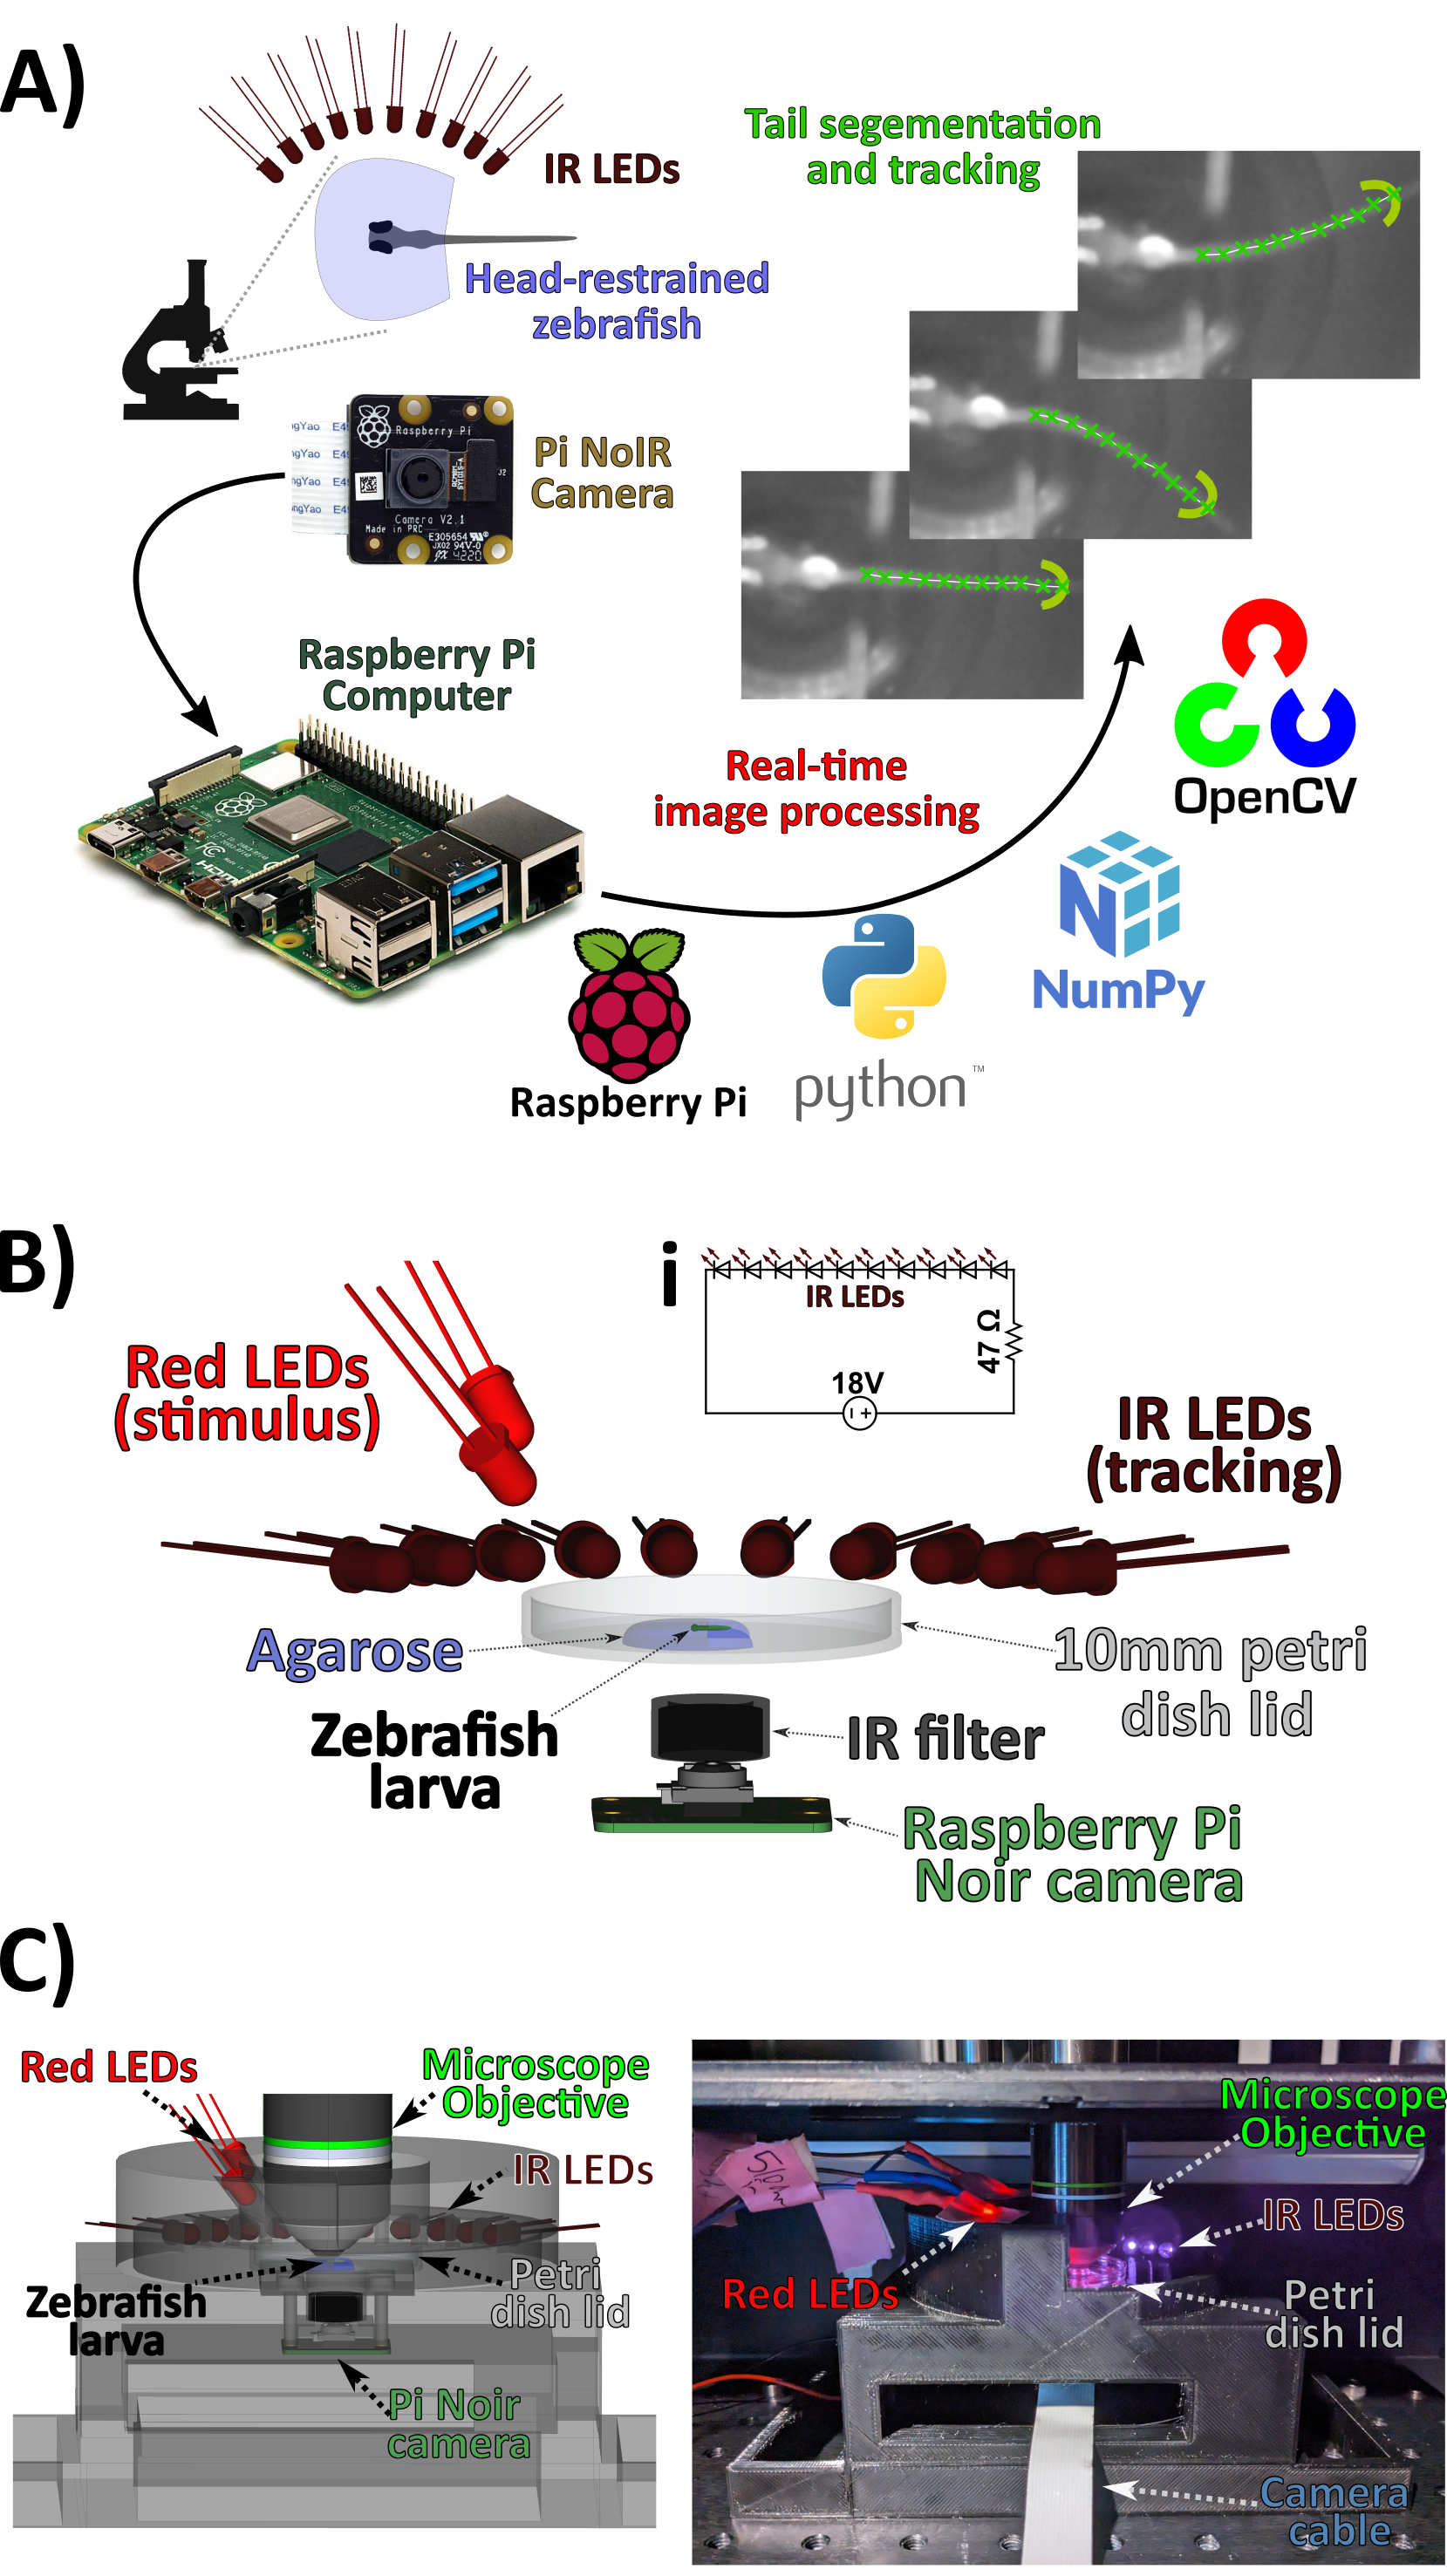
\includegraphics[width=0.58\linewidth]{Figure1_Apparatus.png}
\caption{\textbf{\emph{pi\_tailtrack} apparatus.}
\\ \textbf{A)} The zebrafish larvae being imaged under the microscope is illuminated with infra-red (IR) LEDs, and imaged with the IR-sensitive Raspberry Pi NoIR Camera. Image acquisition and processing is done with a Raspberry Pi Computer and open-source Python packages. The zebrafish tail is identified and segmented in real-time as a sequence of 10 tail segments (green X's). 
\\ \textbf{B)} Rendering of the main components of the apparatus. IR leds illuminate the zebrafish larvae that is head-restrained in agarose in a 35mm diameter petri dish lid. An IR filter blocks the visible stimulus lights (Red LEDs), and the microscope laser from reaching the Raspberry Pi NoIR camera suspended below the fish. \textbf{(i)} Wiring diagram for powering the IR LEDs. 
\\ \textbf{C)} Rendering including the the 3D printed mount and microscope objective. 
\\ \textbf{D)} Annotated photograph of the \emph{pi\_tailtrack} apparatus.  
} 

\label{fig:1}
\end{center}
\end{fullwidth}
\end{figure}

A second challenge is that larval zebrafish move their tails very rapidly, with a tail-beat frequency of between 20-40 hz for normal swimming, which can increase to 100 hz during burst/escape swimming \citep{Budick2000-bq, Muller2004-st, Severi2014-iw}. The V2.1 camera documentation indicates maximum frame rate of 30hz, which is insufficient for imaging tail dynamics. However, by adopting a cropped sensor configuration, and by omitting the JPG compression step in image processing, the camera can be pushed to image at up to 1000hz \citep{660hz}. I adopted a configuration where I imaged with a fixed gain/ISO of 800 in auto-exposure mode, and with a cropped sensor of 128x128 pixels covering 3.5x3.5 mm field of view. This gives sufficient spatial resolution to observe and track the tail of the fish (27 \micro m/px), and most importantly, minimal CPU load. This frees the limited CPU resources on the Raspberry Pi to be used for real-time image processing and tail tracking. 

\subsection{Tail tracking}

Tracking objects in images and videos has undergone a revolution with deep learning and neural network frameworks, where the tracking and reconstruction of complex animal postures is possible after training networks on only a few example images \citep{Mathis2018-rw, Pereira2022-rd}. However, such approaches are computationally intensive and generally require dedicated and GPU hardware beyond the capabilities of the standard Raspberry Pi, making them incompatible with our project goals. In contexts where the image background is predictable and stable, classical computer vision methods like background subtraction, filtering and thresholding may still be preferable to network-based object identification, especially when speed or computational resources are priorities \citep{Mirat2013, Stih2019-gx, Zhu2023}. Here I have used the \emph{Numpy} \citep{harris2020array} and \emph{OpenCV} \citep{opencv_library} libraries to handle the image data and computer vision tasks (\autoref{fig:1}). 

\begin{figure}
\begin{fullwidth}
\begin{center}

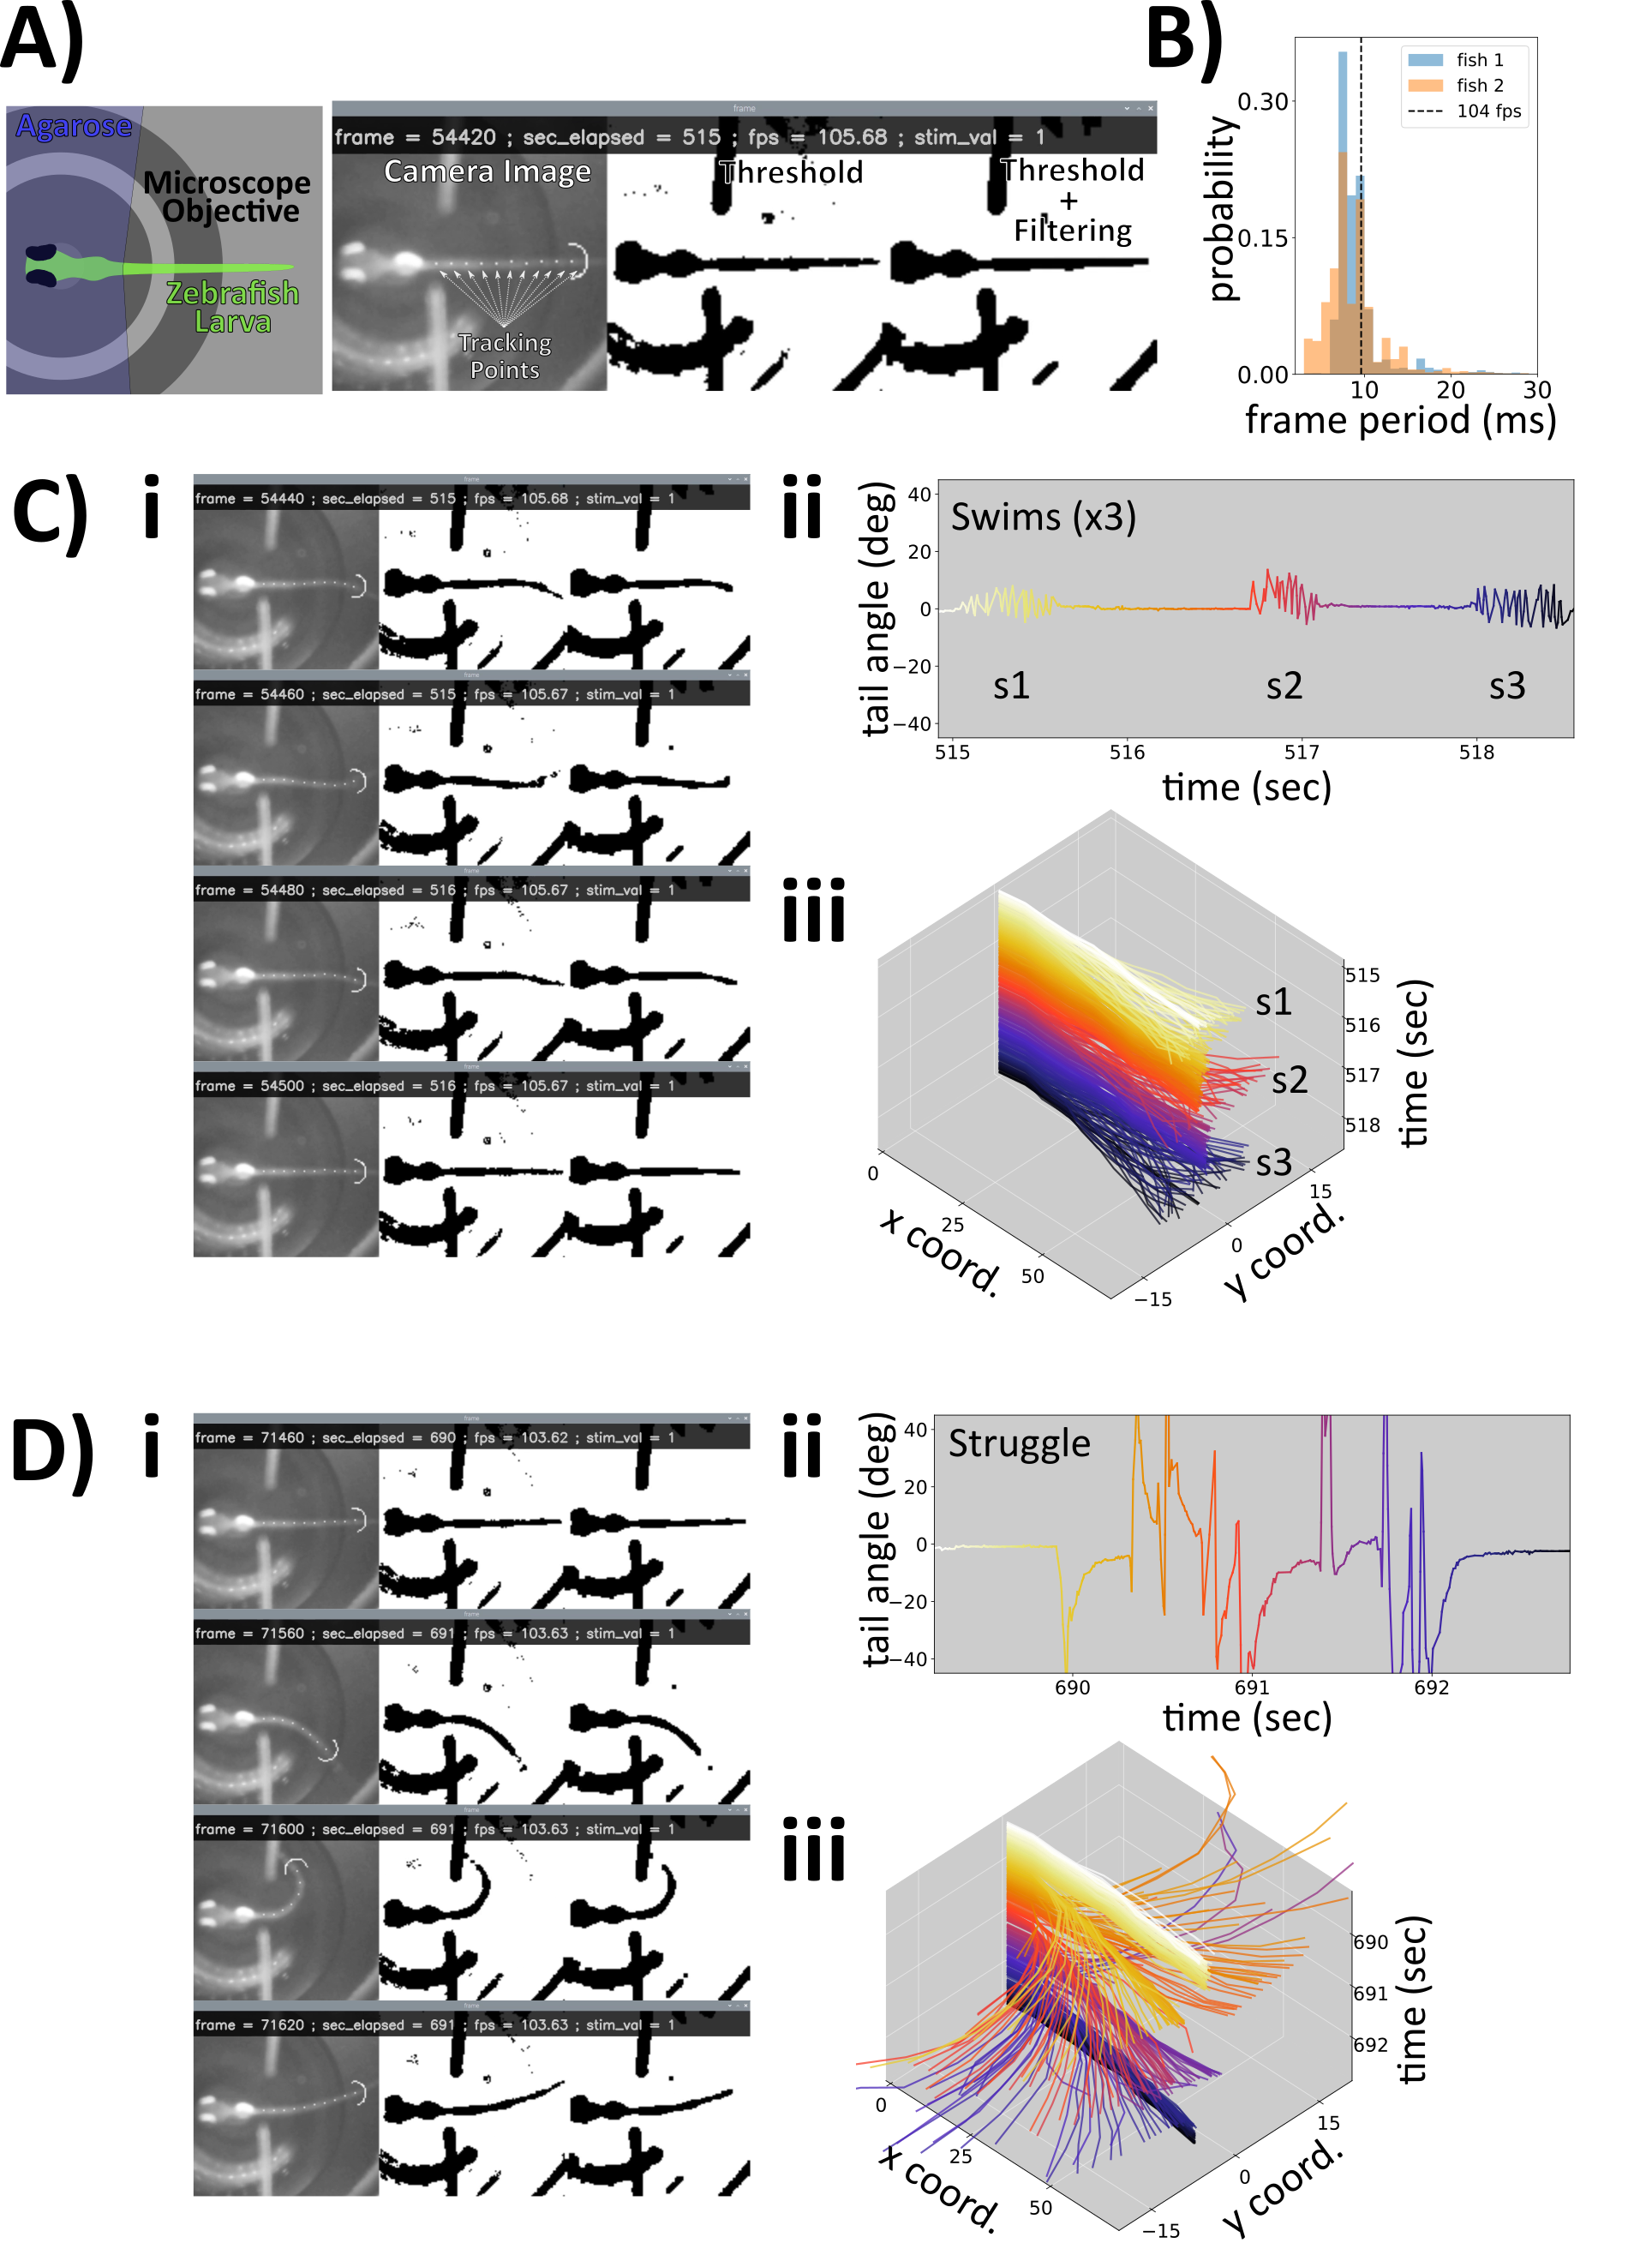
\includegraphics[width=0.65\linewidth]{Figure2_TrackingResults.png}
\caption{\textbf{Larval zebrafish trail tracking examples.}
\\ \textbf{A)} Screenshot of a single frame of a tracking image, showing the image from the camera ("Camera Image") with the resultant tracking points overlayed as white dots. The final tracking point is shown as a white semicircle, which is used in the coordinate search algorithm. "Threshold" shows the result of the Adaptive Thresholding operation, and "Threshold + Filtering" the result of the morphological Opening and Closing operations. Displayed along the top are the: frame (current frame number of the experiment), sec\_elapsed (number of seconds elapsed in the experiment), fps (current frame rate, frames per second), stim\_val (the current value read on the stimulus recording pin: GPIO Pin 4). A schematic of the image field, depicting the agarose mounting medium, the position of the zebrafish, and the microscope objective visible in the background is shown in the left panel.
\\ \textbf{B)} Probability density distribution of individual frame periods from two representative experiments. 
\\ \textbf{C)} i) Example frames during a swimming event. ii) Tail angle deflections during 3 distinct swim events. iii) 3D plot of tail coordinates through the same time period as (ii), drawn in the same time color code. 
\\ \textbf{D)} Same as (C), but for a period in which the larvae executes a struggle/escape maneuver and associated high amplitude tail deflections. 
}
\label{fig:2}

\videosupp{Screen recording of the tail tracking example, \href{https://github.com/owenrandlett/pi_tailtrack/raw/main/SupplementaryVideo_tailtracking_20211213.mkv}{download}}\label{video:S1}


\end{center}
\end{fullwidth}
\end{figure}


I used a computationally lean segmentation and skeletonization strategy (see Materials and Methods) to segment the tail into 10 segments (\autoref{fig:2}), which takes less than 10 ms on the Raspberry Pi CPU. The imaging frame rate when using the \emph{picamera} python package will adjust based on the throughput of the analysis system, which can change with the complexity of the binary images that are processed or external CPU demands, but runs at approximately 104 fps (\autoref{fig:2}B). This is sufficient to clearly distinguish different types of movement events, such as "swims" from "struggles" \autoref{fig:2}C vs. D), and where individual tail beats during swimming events are resolvable. However, this will not be true during rapid/burst swimming, in which tail-beat frequency will exceed our frame rate. If such temporal resolution is required our setup will be insufficient, and we will will only reliably track tail half-beat frequencies of $\leq$50hz. Therefore, this system is not capable of comprehensive behavioural characterization, but can be used to identify different types of swim events. 

During the experiment the software provides a visual display, as is shown in the screenshots in (\autoref{fig:2}), and screen capture video (\autoref{fig:2}--\autoref{video:S1}). Results of the thresholding, filtering, and skeleton tracking are visible and updated in real-time. This can be used to optimize the position of the zebrafish, the Adaptive Thresholding parameters (neighborhood, threshold) using the \emph{'w/a/s/d'} keys, and the position of the first tracking point using the arrow keys.

\subsection{Behavioural analysis of Ca\textsuperscript{2+} imaging data}

\begin{figure}
\begin{fullwidth}
\begin{center}

\includegraphics[width=1\linewidth]{Figure3_FunctionalAnalysis.png}
\caption{\textbf{Identification of behaviour-associated neurons in a larval zebrafish brain via 2-photon Ca\textsuperscript{2+} imaging.}
\\ \textbf{A)} Histogram for the mean tail angle during individual movement bouts for a single larvae over an 80 minute imaging session. Bouts are classified as left or right turns based on a threshold value of 0.004 radians/bout. 
\\ \textbf{B)} Histogram for the bout vigor, quantified using a rolling standard deviation of absolute tail angle. Movements are classified as "swims" or "struggles" based on a threshold value of 0.017 (AU: arbitrary units).
\\ \textbf{C)} Tuning of Ca\textsuperscript{2+} traces in ROIs to turns to the left (green) or right (magenta), as classified in (A). Images are the Pearson correlation coefficient to each behavioral regressor (left or right turns), scaled from 0.0 to 0.3. \emph{Tg2(elavl3:GCaMP6s)} expression pattern is shown in grey. Arrows highlight the Anterior Rhombencaphalic Turning Region (ARTR): with isilateral tuning to turning direction. A = Anterior, P = Posterior
\\ \textbf{D, E)} Tuning of neurons to swims \textbf{(D)}, and struggles \textbf{(E)}, as classified in (B).  
}
\label{fig:3}

\end{center}
\end{fullwidth}
\end{figure}

To test the performance of the \emph{pi\_tailtrack} system, I analyzed Ca\textsuperscript{2+} imaging data from an 80 minute-long volumetric recording covering a large proportion of the brain (as in \cite{Lamire2023-di}). To identify neurons tuned to behavioural parameters I used "regressors" derived from the \emph{pi\_tailtrack} recordings reflecting different motor states convolved with the GCaMP response kernel (as in \cite{Miri2011-sr}). Zebrafish swim bouts can be classified as either forward swims or turns, and an area within the anterior hindbrain is associated with turning direction. This area is known as the Anterior Rhombencephalic Turning Region (ARTR: \cite{Dunn2016-bg}, also called the HBO: \cite{Ahrens2013-xh, Wolf2017-ma}), and shows a conspicuous activity pattern with stripes of neurons tuned to the ipsilateral turning direction. By looking at correlations to regressors reflecting right and left turns, I identified these stripes of neurons in the ARTR-region, indicating that I can successfully identify the ARTR using \emph{pi\_tailtrack} (\autoref{fig:3}A,C). A similar analysis looking at "swims" vs "struggles", with "struggles" reflecting high-amplitude tail flicking events (\autoref{fig:2}D, \autoref{fig:3}B), identified differential neuronal activation in the context of these two movement categories (\autoref{fig:3}D,E), with the presence of lateral hindbrain populations of neurons that were negatively correlated with "swims", and a broader and more positively correlated population with "struggles". 


\subsection{Future developments}

Here I have used the \emph{pi\_tailtrack} system to simply record the behaviour of the animal independent of the microscopy or any stimulus delivery. Therefore, the timing of microscope image acquisition is controlled by the microscope computer and is independent of \emph{pi\_tailtrack}. These separate experimental clocks (microscope frames vs Pi Camera frames) must be synchronized, and in our case I have used the GPIO input pin on the Raspberry Pi to record the timing of the stimuli delivered by the microscope relative to the Pi Camera frames. An alternative solution would be to use the Raspberry Pi to deliver the stimuli, perhaps by integrating a video projector system to allow for the delivery of arbitrary and complex visual stimuli. This would also open up possibilities for performing "virtual reality" experiments, where the behaviour of the animal dictates the stimulus in closed-loop. In some microscope systems it should also be possible to use the Raspberry Pi GPIO to trigger microscope acquisitions. This may be preferable if the synchronization between imaging and behaviour frames is critical. 

It is also important to note that hardware in this micro-computer/Raspberry Pi space is rapidly evolving. Indeed, a new suite of Raspberry Pi V3 Cameras have just been released, offering increased resolution, dynamic range, and frame rate. Using these cameras, we may be able to increase the frame rate of tracking into the multiple-hundreds of hz, which would allow us to more reliably resolve individual tail half-beats. The Raspberry Pi "Global Shutter" Camera has also recently been released, which is likely also going to be very interesting for behavioural neuroscience, as the use of a global shutter avoids rolling shutter artifacts that distort images along the frame during rapid motion. The software introduced here could be further optimized for speed/framerate, for example by moving to a multi-threaded architecture to distribute the image acquisition and tracking computations \citep{Zhu2023, Randlett2019-fj}, using a compiled language (e.g.  C/C++ or Julia), or perhaps by moving image processing onto the Raspberry Pi GPU. 

\subsection{Conclusion}

Here I described our system for tracking the tail of the larval zebrafish during microscopy. Many of the practical considerations of this setup may be specific to our application, and therefore may need modification for use in other experiments in other labs. However, I feel that the core and simple idea of using an IR-sensitive Raspberry Pi Camera, a simple Python script, coupled with IR LEDs and and IR filter, provides an approachable and flexible solution that may be widely useful for observing and tracking the behaviour of zebrafish (or perhaps other animals) while performing imaging experiments. This system's attributes may also make it an ideal tool for community engagement activities such as school outreach programs. It could serve as a platform for learning about microelectronics, behavioural analyses, machine vision, and hardware design and construction.

\section{Funding}

This work was supported by funding from the ATIP-Avenir program of the CNRS and Inserm, a Fondation Fyssen research grant, and the IDEX-Impulsion initiative of the University of Lyon.

\section{Data Availability}

Software and analysis code is available here:  \href{https://github.com/owenrandlett/pi_tailtrack/}{https://github.com/owenrandlett/pi\_tailtrack/}. Datasets are available here: \href{https://www.dropbox.com/sh/dbjq2dud1ws1o2v/AACLamthISys8sUD1a5oRcR1a?dl=0}{pi\_tailtrack datasets}.

\bibliography{References_HabEstrogen}

\end{document}
supplement